\documentclass[a4paper, 12pt, twoside]{article}
\usepackage{microtype}
\usepackage{tikz}
    \usetikzlibrary{svg.path}
    \usetikzlibrary{positioning, shapes.geometric, arrows}
\usepackage[T1]{fontenc} % https://tex.stackexchange.com/a/392210 polskie znaki
% \usepackage[polish]{babel}
\usepackage{indentfirst}
\usepackage{todonotes}
\usepackage[breaklinks]{hyperref} % Citation to bibliography linking
\usepackage[
    backend=biber,
    style=numeric-comp,
    sorting=none
]{biblatex}
\addbibresource{bibliografia.bib}
\usepackage{cprotect} % escape \verb in hrefs and footers
\usepackage{graphicx}
\usepackage{float}
\graphicspath{ {./images/} }
\usepackage{geometry}

\renewcommand*\contentsname{Spis treści}
\renewcommand*\figurename{Rysunek}
\renewcommand*\listfigurename{Spis rysunków}


\begin{document}
    \renewcommand{\maketitle}{
    \begin{titlepage}
    \begin{center}
        \textbf{UNIWERSYTET ŚLĄSKI W KATOWICACH\\
        WYDZIAŁ NAUK ŚCISŁYCH I TECHNICZNYCH\\
        }

        \vspace{1.5 cm}
        
        \Large 
        Kacper Hałaczkiewicz\\
        Nr albumu: 338889\\
        
        \vspace{0.5 cm}
        
        Przygotowanie kompletnego rozwiązania CI/CD \\
        na podstawie aplikacji z .NET MAUI
        
        \vspace*{2.0 cm}
    
        \small
        PRACA DYPLOMOWA INŻYNIERSKA\\
        
        \vspace{8.0 cm}
    
        \large
        Promotor: dr hab. Arkadiusz Bubak\\
        
        \vspace{1 cm}
        
        \small 
        Katowice 2024\\
    \end{center}
    \clearpage
    \end{titlepage}
}

\maketitle



    % \section{Streszczenie}

W niniejszej pracy opisuję główne założenia i implementację zautomatyzowanego 
procesu wydawczego oprogramowania na przykładzie multiplatformowej aplikacji.
Znajdziemy w niej zarówno objaśnienie architektury oprogramowania, 



    
    \tableofcontents

    \section{Wstęp}
% Co w pracy znajdziemy
    % Skrót informacji potrzebnych do zrozumienia pracy
    % Działająca aplikacja multiplatformowa
    % Instrukcja utworzenia funkcjonującego piepline'a
% Czego w pracy nie znajdziemy
    % Dogłębnej analizy działania biblioteki do pathfindingu (wyłącznie linki)

Założeniem pracy jest stworzenie kompletnego rozwiązania w postaci \\ 
aplikacji ułatwiającej
nawigowanie po budynku Śląskiego Międzyuczelnianego Centrum Edukacji i Badań Interdyscyplinarnych (SMCEBI),
oraz zautomatyzowanego środowiska kompilującego i dystrybuującego rozwiązanie.

    W mojej pracy zawarłem krótkie objaśnienia terminów, których zrozumienie jest bardzo przydatne
(a czasem nawet kluczowe) do uruchomienia mojego rozwiązania. Najciekawsze źródła, których nie cytowałem,
ale odwiedziłem i naprowadziły mnie na poprawne tory bądź rozwijają temat umieściłem w rozdziale


    Podczas tworzenia programu skorzystałem z gotowej biblioteki do wyznaczania ścieżek,
wobec czego w niniejszej pracy znajduje się wyłącznie skrócone wytłumaczenie schematu działania
jej algorytmu.

    \section{Objaśnienie zastosowanych narzędzi i technik programistycznych}

\subsection{.NET MAUI} \label{mauiFrameworkSubsection}
.NET MAUI \cite{mauiDefinition} to platforma programistyczna (ang. framework) umożliwiająca
kompilację natywnych aplikacji wieloplatformowych. Jest to następca Xamarina~\cite{xamarin},
czyli poprzedniego rozwiązania Microsoftu do tych samych zastosowań.

Najważniejszą różnicą jest obsługa projektów - Xamarin wymagał osobnych projektów na każdy system operacyjny, 
zaś MAUI obsługuje je wewnątrz jednego, uniwersalnego projektu.

Framework umożliwia skorzystanie z uniwersalnych kontrolek i interfejsów, 
które na etapie kompilacji są tłumaczone na natywne odpowiedniki każdej z platform. 
Takie rozwiązanie pozwala na skupienie się na tworzeniu zawartości aplikacji,
stworzenie ogólnego zarysu w bardzo krótkim czasie, jednocześnie nie rezygnując z multiplatformowości.

\subsection{Microsoft Azure} \label{MS_AzureSection}
Microsoft Azure \cite{azure} to internetowa platforma oferująca szeroki wachlarz narzędzi i usług
z zakresu tworzenia, rozwoju i dystrybucji oprogramowania. Za jej pomocą możemy wynająć moc obliczeniową
w chmurze Microsoftu - począwszy od baz danych, aż po maszyny wirtualne. Platforma oferuje również
pełne środowisko programistyczne - DevOps Server, które wspomagaja komunikację, 
formalizujące wprowadzane zmiany, automatycznie testuje, integruje i dystrybuuje rozwiązania.

\subsection{MVVM} \label{mvvmSubsection}
MVVM to akronim Model-View-Viewmodel (w tłumaczeniu Model - Widok - Model widoku), czyli programistycznego wzorca projektowego. \\
Polega na wprowadzeniu separacji pomiędzy modelem danych i sposobem ich obróbki, widokami je reprezentującymi oraz operacjami pomiędzy nimi. \\
Jego główną zaletą jest możliwość oddzielenia ogólnych założeń programu od szczegółów integracji z platformą 
- w projekcie~\cite{Halaczkiewicz_Navigator_GitHub} jest to wyraźnie zarysowane dzięki przyjętej 
konwencji nazewniczej plików (postfix -Model, -ViewModel lub -View).
% Na Rys.~\ref{fig:MVVM_diagram} możemy zaobserwować zależność komunikacji klas stworzonych z wykorzystaniem właśnie tego wzorca.
% \begin{figure}[!htp]
%     \centering
%     \begin{tikzpicture}[
%         minimum height=1cm,
%         block/.style={rectangle, draw=black!60, fill=green!30, thick, rounded corners=2mm}
%         ]
%             \node[block] (Model) {Model};
%             \node[block] (ViewModel) [right=of Model] {ViewModel};
%             \node[block] (View) [right=of ViewModel] {View};
            
%             \draw[->] (Model.east) -- node[anchor=east]{} (ViewModel.west);
%             \draw[->] (ViewModel.east) -- node[anchor=east]{} (View.west);
%     \end{tikzpicture}
%     \caption{Zależności między klasami w MVVM~\cite{mvvm}}
%     \label{fig:MVVM_diagram}
% \end{figure}


    \section{Aplikacja ,,Navigator''} \label{NavigatorAppSection}

Chociaż w założeniach mojej pracy inżynierskiej może być odebrana wyłącznie jako implementacyjny szczegół, 
to uważam, że warto pochylić się nad procesem tworzenia, wykorzystanymi narzędziami i technikami
oraz sposobem działania opisanej poniżej aplikacji.

\subsection{Przedstawienie aplikacji}

Aplikacja Navigator służy do tworzenia i przeglądania planów\\%
wielopiętrowych budynków.
Za jej pomocą Użytkownik może skorzystać z wcześniej przygotowanych map lub utworzyć własną za pomocą kreatora.
Do jej stworzenia wykorzystałem bibliotekę Leaflet~\cite{leafletGithub}, 
która pozwala na wyświetlanie mapy w postaci strony HTML za pomocą JavaScript.

W zrozumieniu jej działania, nieopisaną pomocą okazał się projekt Floorplans~\cite{floorplansGithub},
na jego podstawie byłem w stanie wstępnie sprawdzić zachowanie przeglądarkowych kontrolek, 
a następnie za pomocą inżynierii wstecznej zaimplementowałem podstawowy interfejs biblioteki, 
czyli \verb|LeafletAPI|.

\newpage

\subsection{Zastosowanie .NET MAUI}

.NET MAUI pozwala na użycie logiki programu na różnych platformach (w przypadku mojej pracy Android oraz Windows).
Każdy element interfejsu jest stworzony i wyświetlany zgodnie z natywnymi elementami, 


\newpage

\subsection{Architektura aplikacji}

\subsubsection{Wzorce projektowe}
\paragraph{Wzorzec MVVM}
W aplikacji starałem się korzystać ze wzorca projektowego MVVM~\ref{mvvmSubsection} - 
wprowadziłem podział na odpowiednio:
\begin{itemize}
    \item Pliki znaczników - strona\verb|.xaml|
    \item Code-behind (kodu związanego bezpośrednio z danym widokiem) - strona\verb|.xaml.cs|
    \item ViewModel, który jest przygotowany dla każdego widoku - strona\verb|ViewModel.cs|
    \item Modele, przechowywane w specjalnym folderze \verb|Models| oraz ujęte w odrębnej przestrzeni nazw
\end{itemize}

Zamysł polega na umożliwieniu bezpośrednich interakcji danych 
modelowych wyłącznie z ViewModelami. Takie podejście umożliwia bezpieczną zmianę 
widoków, bez zastanawiania się czy wpłyną one na zachowanie ViewModelu lub co gorsza wprost na dane.

\paragraph{Wzorzec "Budowniczy"}
Tworzenie obiektu mapy postanowiłem rozwiązać za pomocą wzorca Buildera - 
specjalna klasa MapBuilder krok po kroku 


\subsubsection{Podział na projekty}
Oprócz bezpośredniego kodu aplikacji, zdecydowałem się na wyodrębnienie 3 projektów:

\paragraph{NavigatorTests}
Projekt służący do statycznej analizy kodu poprzez przeprowadzenie testów jednostkowych.
Nie jest on obszerny, ale wraz z rozwojem oprogramowania może znaleźć się w nim więcej 
scenariuszy. Na potrzeby tej pracy został zaimplementowany jeden test pokazowy, 
żeby móc skonfigurować ich wywołanie za pomocą pipeline'a.

\paragraph{MapBuilder\_API\_Base}
Projekt definiuje interfejs \verb|IMapBuilder|, który należy zaimplementować przy dodawaniu 
do aplikacji biblioteki wyświetlającej mapę, tak jak stało się to w przypadku LeafletAPI.
Ten podział wprowadza kompatybilność i możliwość zmian minimalnym kosztem programistycznym.

Aby dodać swoją bibliotekę należy \todo{Rozważyć zmiany w programie aby nie przekompilowywać Navigatora}

\paragraph{LeafletAPI}
W projekcie zaimplementowałem generowanie strony HTML z wykorzystaniem wspomnianej biblioteki Leaflet~\cite{leafletGithub}.
Biblioteka tworzy obiekt \verb|MapBuilder| implementujący interfejs \verb|IMapBuilder|, który jest 
za pomocą aplikacji poszerzany o kolejne piętra, pokoje oraz obiekty z kreatora, a po wywołaniu 
metody \verb|Build| zwraca wynikowy skrypt, który zostaje zwrócony do aplikacji.

W zrozumieniu działania biblioteki, nieopisaną pomocą okazał się projekt Floorplans~\cite{floorplansGithub},
na którego podstawie byłem w stanie wstępnie sprawdzić zachowanie przeglądarkowych kontrolek, 
a następnie za pomocą inżynierii wstecznej zaimplementować jego funkcjonalność w uniwersalny sposób.



    
    \section{Narzędzia CI/CD}

\subsection{Wprowadzenie}
Zaraz po stworzeniu software'u, najważniejszym etapem jest możliwość szybkiego i bezpiecznego dostarczenia go do odbiorców.
W najmniejszych projektach po skompilowaniu aplikacji zazwyczaj wystarczyło skopiowanie plików
i przeniesienie ich na końcowe urządzenie. O ile jest to najprostsze i najbardziej oczywiste rozwiązanie,
jest ono zdecydowanie najmniej wydajne na dłuższą metę.

Wydanie nowej wersji programu możemy w uproszczony sposób przedstawić jako cykl na poniższym rysunku~\ref{fig:cyklZmian}.
Za każdym razem gdy zostaną wprowadzone jakiekolwiek zmiany, należy przygotować nową wersję (kompilacja),
umieścić ją w odpowiedniej lokalizacji (czy to będzie sklep z aplikacjami, strona internetowa czy nośnik cyfrowy),
a następnie poinformować o tym użytkownika (przykładowo wyświetlić powiadomienie o dostępności aktualizacji).


\begin{figure}[!htp]
    \centering
    \begin{tikzpicture}[
        minimum height=1cm,
        block/.style={rectangle, draw=black!60, fill=green!30, thick, rounded corners=2mm}
        ]
            \node[block] (codeChange) {1. Wprowadzenie zmian w kodzie};
            \node[block] (compilation) [right=of codeChange] {2. Kompilacja rozwiązania};
            \node[block] (publish) [below=of compilation] {3. Publikacja plików};
            \node[block] (newVerInfo) [below=of codeChange] {4. Poinformowanie o nowej wersji};

            \draw[->] (codeChange.east) -- node[anchor=east]{} (compilation.west);
            \draw[->] (compilation.south) -- node[anchor=south]{} (publish.north);
            \draw[->] (publish.west) -- node[anchor=west]{} (newVerInfo.east);
            \draw[dotted] (newVerInfo.north) -- node[anchor=north]{} (codeChange.south);
            
    \end{tikzpicture}
    \caption{Uproszczony proces wydawania nowej wersji oprogramowania}
    \label{fig:cyklZmian}
\end{figure}

Wraz ze wzrostem częstotliwości wprowadzania zmian, ilości urządzeń oraz ograniczeniem dostępu do nich,
potrzeba automatyzacji tego procesu staje się coraz bardziej realna. 
W tym celu wykorzystuje się szeroki wachlarz narzędzi CI/CD. \todo{}

\subsection{Czym jest CI/CD?}
Angielskie \textbf{\textit{Continous Integration / Continous Delivery}} (czyli ciągła integracja i dystrybucja oprogramowania) 
to określenie na zestaw narzędzi automatyzujących dostarczanie programów wraz z ich rozwojem. 
Pełne rozwiązanie, które samodzielnie wypełnia wszystkie nasze kroki wydawcze, nazywamy \textbf{\textit{pipeline}}m (z ang. rurociąg).
Jego istotą jest zapewnienie wydajnego i stabilnego przepływu danych w ramach wypracowanej listy kroków, 
które każdorazowo zostaną wykonane w ten sam sposób~\footnote[1]{
    \label{determinismFootnote}
    Z dokładnością do środowiska, w którym skrypt zostanie uruchomiony, 
    oraz sposobu działania narzędzi (Patrz determinizm kompilatora~\cite{compilerDeterminism})
}, aby otrzymać zamierzony efekt.

\subsubsection{Zalety Pipeline'ów}
Do jego zalet zaliczamy:
\begin{itemize}
    \item Wyeliminowanie błędów i niedopatrzeń człowieka na etapie wydawczym
    \item Przyspieszenie działania procesu
    \item Zwiększenie dostępności 
    \item Determinizm wydania~\footref{determinismFootnote}
    \item Uproszczona analiza szczegółów procesu
    \item Odciążenie zespołu programistycznego z wiedzy o szczegółach procesu wydania
    \item Bezpieczeństwo
\end{itemize}

O ile sam pipeline możemy przedstawić i wykonać jako skrypt terminalowy, 
to jednak dysponujemy już nowoczesnymi narzędziami, które wprowadzają kolejny poziom abstrakcji.
U podstaw są to dokładnie takie same wywołania z linii poleceń, ale opakowanie ich w interfejs graficzny 
lub prostszy język (najczęściej jest to YAML~\cite{yamlDefinition}) upraszcza ich konfigurowanie, 
obniża trudność uczenia się ich obsługi oraz zazwyczaj pozwala na szybszą analizę wyników ich wywołań.

Jako przykład takiego zadania możemy podać skorzystanie .NET Core SDK - o ile musimy poznać możliwości SDK,
to wywołanie ręczne przekazywanie danych wejściowych do terminala zostaje zastąpione modułem, 
dzięki któremu jesteśmy odciążeni z wpisywania słów kluczowych, a jedynie wybieramy je z rozwijanej listy 
lub opisujemy nasze wymagania w skrótach.

Ważnym aspektem jest również bezpieczeństwo - wrażliwe dane, takie jak certyfikaty używane do podpisywania aplikacji czy
hasła dostępowe do serwerów powinny być udostępnione jak najmniejszej ilości osób.

W momencie gdy każdy z deweloperów uaktualnia aplikację ręcznie, musi dysponować tymi informacjami,
zaś korzystając z pipeline'a taki dostęp mają wyłącznie wyselekcjonowane osoby zarządzające procesem.
Zmniejszenie dostępności tych informacji sprawia, że ryzyko wykradnięcia tych danych jest niemal zerowe.

Przykładowo duża firma, która tworzy popularną przeglądarkę internetową, zostaje okradnięta z certyfikatów i haseł - 
będąc w posiadaniu tak istotnych danych, ktoś może stworzyć własną aplikację, która przykładowo wykrada personalia użytkowników, 
a następnie podszyć się pod prawdziwą aplikację. 
Tego rodzaju straty prowadzą do bardzo poważnych konsekwencji, na co nie możemy sobie pozwolić.

\subsubsection{Kompromisy i wady}
Istnieje kilka zagadnień, które należy rozważyć podczas planowania integracji pipeline'a z naszym projektem:
\begin{enumerate}
    \item Ilość czasu potrzebnego do przygotowania konfiguracji
    \item Czy pipeline ma działać w chmurze, czy na własnym urządzeniu
\end{enumerate}

Zwykle przygotowanie konfiguracji pipeline'a jest skomplikowane oraz \\%
czasochłonne, więc do tego zadania zatrudnia się specjalistów\todo{}. \\
Chociaż początkowo może wydawać się to zbędnym nakładem pracy, z upływem czasu zwraca się on z nawiązką.
Jeżeli nasz projekt ma być rozwijany przez więcej osób, w większej perspektywie czasowej, 
to oprócz jego standardowych zalet, zyskujemy również spokój współautorów, 
którzy nie muszą znać szczegółów procesu wydawczego i mogą skupić się na tworzeniu jego zawartości.

Spotkałem się z opiniami, że przywiązanie do jednego dostawcy narzędzia negatywnie wpływa na elastyczność 
takiego pipeline'a - w przypadku potrzeby zmiany narzędzia CI/CD mogą pojawić się komplikacje, 
przykładowo różnice w składni, limity przechowywania poufnych danych, sposób działania~\footnote[2]{
    Niekompatybilność przekazywania zmiennych, konwencje nazewnicze, dostępność szablonów zadań
} itp.
Aby zabezpieczyć się przed takimi trudnościami, należy przeznaczyć dodatkowe nakłady pracy na stworzenie 
modularnych skryptów, które będą łatwe w użyciu.
Sprawa sekretów jest znacznie bardziej skomplikowana - większość firm stosuje mechanizmy uniemożliwiające pobranie już 
zabezpieczonych danych, więc o ile nie przechowujemy ich kopii samodzielnie, może okazać się to istotnym utrudnieniem w migracji.

W zależności od naszych możliwości finansowych oraz zaopatrzeniowych, możemy wynająć maszynę wirtualną
lub zainstalować odpowiednie oprogramowanie CI/CD na własnej maszynie. 
Jeżeli wolimy nie martwić się o sprawy sprzętowe, wygodniejszym rozwiązaniem jest chmura,
ale jeśli dysponujemy sprzętem, to prawdopodobnie skorzystanie z niego będzie tańszą opcją. 
\todo[size=\scriptsize]{czy ja to muszę jakoś potwierdzać? czy to wystarczy?}



\subsection{Dostępne systemy CI/CD}

Jenkins

TeamCity

GitHub Actions 

BitBucket Pipelines

\subsection{Kontrola wersji}

Jedną z najważniejszych części CI/CD są systemy kontroli wersji. 
W przypadku współpracy nad kilkuosobowym projektem, ogromnym rozwiązaniem 
we wiodącej firmie czy nawet pracując samemu - możliwość cofnięcia konkretnych zmian, 
sprawdzenia historii poprawek aby poznać lub przypomnieć sobie ich kontekst, 
jak również aby sprawdzić w jaki sposób coś działało wcześniej - każdy z tych scenariuszy 
mógłby być zastąpiony zwykłą kopią zapasową. 
Ze względu na optymalizację czasowo-kosztową (szybkość działania, 
wygodę obsługi, optymalizację zajmowanego miejsca) znacznie lepszym systemem są dedykowane 
rozwiązania, takie jak Subversion (SVN), CVS czy opisany niżej (prawdopodobnie najpopularniejszy) Git.

W dużym skrócie, Git jest systemem kontroli wersji, charakteryzującym się:
\paragraph{Rozproszeniem repozytoriów -}
Pobierając aktualną wersję kodu, najczęściej wykonujemy również pełne sklonowanie repozytorium, 
co częściowo uodparnia system na ewentualne utraty efektów pracy przez awarie sprzętowe lub pomyłki.
Możemy również cofać się w historii wersji bez wielokrotnego kontaktowania się z serwerem.

\paragraph{Zaoszczędzenie przestrzeni dyskowej -}
Mechanizm różnicowego przechowywania danych pozwala na zmniejszenie rozmiaru plików, 
wciąż zachowując możliwość dostępu do ich wcześniejszych wersji.
Zamiast wielokrotnie nieznacznie zmieniony plik w całości, wystarczy notować w którym miejscu 
wprowadziliśmy jakie zmiany. Jest to metoda mniej wydajna obliczeniowo, ponieważ każde cofnięcie się 
o konkretną ilość wersji prowadzi do inkrementacyjnego odtworzenia informacji, 
ale jest to na tyle mały narzut pracy względem zaoszczędzonej przestrzeni dyskowej, że w połączeniu 
z prędkością aktualnych komputerów jest to bardziej opłacalna metoda~\cprotect\footnote{%
    Oczywiście istnieją specjalne mechanizmy pozwalające na optymalizację tego zachowania, 
    dobrym punktem wyjścia jest \verb|git maintenance|~\cite{gitMaintenance}}.

\paragraph{Uproszczeniem pracy zespołowej -}
System branchy (z ang. gałęzi, odgałęzień) pozwala na odesparowanie konkretnych funkcjonalności, 
podzielenia fragmentów pracy na etapy, jak również na wygodne odseparowanie środowisk pracy deweloperów.
Nie każda osoba musi pobierać wszystkie odgałęzienia, nie mamy ograniczeń ilościowych lub wielkościowych 
jeżeli chodzi o wprowadzane zmiany. Możemy zacząć nad czymś pracować, ale jeżeli będziemy chcieli tymczasowo 
wstrzymać lub porzucić prace, możemy niemalże bez konsekwencji odłożyć je na później i zacząć wdrażać 
inne funkcjonalności.\\%
Po zakończeniu pracy w danym branchu, możemy z powrotem włączyć go do współdzielonej części - następuje 
wtedy specjalne porównanie zmian, które w większości wypadków pozwala na automatyczne ich połączenie, 
a w razie bardziej skomplikowanych niuansów łatwo rozwiejemy wątpliwości w specjalnym narzędziu.

\subsubsection{Integracje międzysystemowe}
Platformy oferujące usługi hostingowe (takie jak zastosowany w tej pracy GitHub~\cite{github}) oferują 
ogromną gamę integracji najróżniejszych narzędzi i systemów - począwszy od możliwości importu 
repozytoriów, nienadzorowanego udostępniania jego zawartości, powiadomienia o zmianach przez najróżniejsze 
kanały informacyjne (WebHooki, RSS, powiadomienia i e-maile), jak również dostęp do wielu innych 
funkcjonalności jak narzędzia upraszczające i formalizujące kontakt z zespołem 
lub podstronie wydawczej, takiej jak GitHub Releases~\cite{githubReleases}.

GitHub Releases to specjalny mechanizm, pozwalający na opublikowanie gotowych rozwiązań, dostępnych do 
pobrania w gotowej do użytku formie. Na Rys.~\ref{img:githubReleases_sample} możemy zobaczyć 
przykładowe wydanie wersji programu - zawiera tytuł (lub w tym przypadku numer wersji), listę zmian 
oraz co najważniejsze skompilowane pliki wraz z ich ekwiwalentnym kodem źródłowym.
\begin{figure}[ht]
    \centering
    \frame{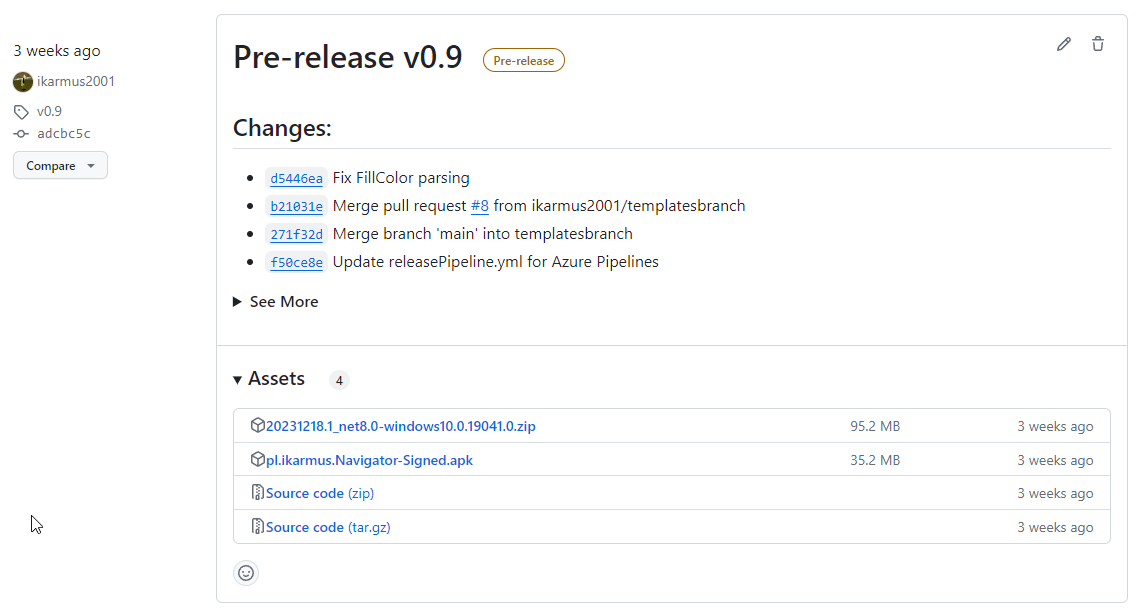
\includegraphics[width=0.9\textwidth]{githubReleases_sample.png}}
    \caption{Przykładowe wydanie aplikacji w GitHub Releases}
    \label{img:githubReleases_sample}
\end{figure}

W moim projekcie skorzystałem również z opcji triggerów (ang. wyzwalaczy), które powiadamiają 
połączone usługi o zmianach w kodzie. \\%
Wysłanie kolejnego commita na określony branch powiadamia 
Azure o tym fakcie, co skutkuje zakolejkowaniem nowego uruchomienia pipeline'a.

\subsection{Implementacja}
W mojej pracy zdecydowałem się na skorzystanie z platformy Azure~\ref{MS_AzureSection} - 
wpłynęły na nią przyjazny interfejs, łatwość instalacji agenta, jasna struktura tworzenia pipeline'ów 
oraz mnogość instrukcji i poradników dotępnych w Internecie.

Na przykładzie aplikacji ,,Navigator''~\ref{NavigatorAppSection} chciałbym przedstawić proces \\
planowania i konfiguracji pipeline'a.

\subsubsection{Określenie potrzeb i możliwości}
W moim projekcie, oprócz samej kompilacji, postanowiłem zaimplementować etap testowania 
oraz wydania aplikacji na wspomnianym wcześniej GitHub Releases~\cite{githubReleases}.
Na Rys.~\ref{img:JobsOverview} widzimy efekt wykonania takiego pipeline'a z poziomu 
widoku zarządzania pipeline'ami na stronie Microsoft Azure:

\begin{figure}[ht]
    \centering
    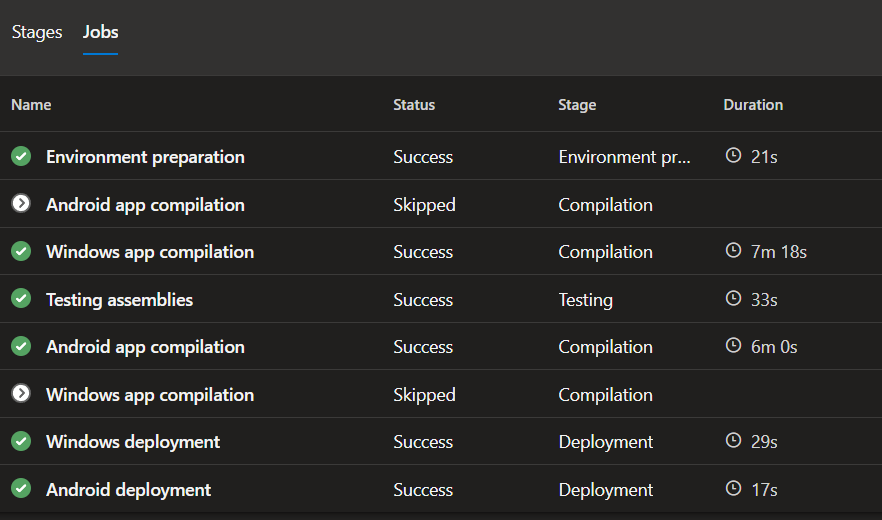
\includegraphics[scale=0.5]{JobsOverview.png}
    \caption{Zadania (ang. joby) wykonane przez pipeline}
    \label{img:JobsOverview}
\end{figure}

\subsubsection{Przygotowanie środowiska kompilacyjnego}
Pierwszym krokiem było zainstalowanie specjalnego oprogramowania, 
które wykonuje wszystkie kroki zdefiniowane w pipelinie - Azure Build Agent~\footnote{
    \href{https://learn.microsoft.com/en-us/azure/devops/pipelines/agents/agents}{
        Informacje o Agentach
    }
}.
Ze względu na dysponowanie własną, dostępną maszyną zdecydowałem się na tą opcję,
jednak taki sam efekt można osiągnąć opłacając maszyny wirtualne, udostępniane przez Microsoft.

Po krótkiej konfiguracji Agent był gotowy do wykonywania zleconego pipeline'owego skryptu, 
ale należało jeszcze dodać zmienne środowiskowe, które pozwalają na 
skorzystanie z określonych funkcji zadań (przykładowo użycie Javy - paragraf \ref{javaTask}).

\subsubsection{Zdefiniowanie wymaganych akcji}
Utworzenie pakietu mojej aplikacji napisanej w .NET MAUI przebiega za pomocą wywołania kompilatora 
\verb|dotnet| z opcją \cprotect{\href{https://learn.microsoft.com/en-us/dotnet/core/tools/dotnet-publish}}{\verb|publish|}, 
która uruchamia przywrócenie wszystkich zależności (\verb|restore|), 
kompiluje ją (\verb|build|) oraz pakuje do przewidzianego w konfiguracji projektu (\verb|.csproj|) formatu~\cprotect\footnote{%
    Interesującym może okazać się fakt, że aplikację w .NET MAUI kompilujemy w oparciu o projekt, a nie rozwiązanie (\verb|.sln|).
    Jest to spowodowane kolejnością interpretacji plików
}.

Zdecydowałem się na podpisywanie aplikacji osobnym zadaniem ze względu na modularność,
jak również ze względu na chęć ominięcia szczegółów tej operacji wewnątrz samego kodu (tj. w pliku projektu).

\subsubsection{Podejście graficzne}
Moja pierwsza próba konfiguracji została podjęta w ramach graficznego konfiguratora, 
który pozwolił mi na wykonanie (jak się później okazało szkicu) mojego pipeline'a.
Na Rys.~\ref{img:PipelineGuiApproach} i \ref{img:taskGroupMauiPrepare} możemy zobaczyć jego schemat działania:

\begin{figure}[ht]
    \centering
    \begin{minipage}[t]{0.5\textwidth}
        \centering
        \frame{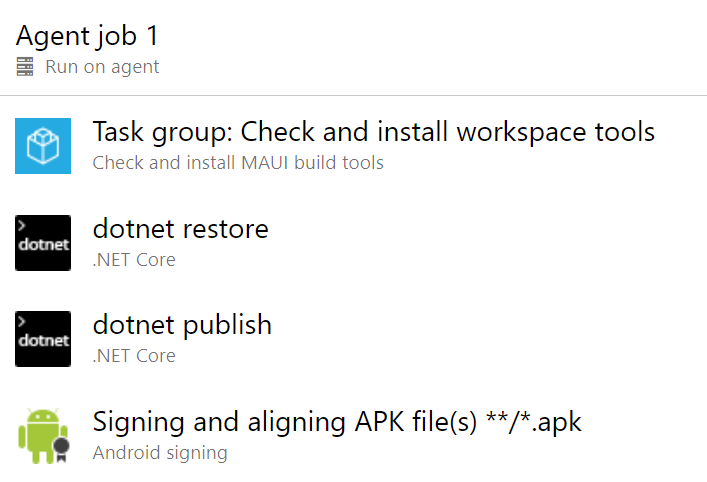
\includegraphics[width=\textwidth]{PipelineGuiApproach_light.png}}
        \caption{Grupa zadań inicjujących środowisko 
            (szczegóły na Rys.~\ref{img:taskGroupMauiPrepare}) 
            oraz publikacja i podpisanie cyfrowe}
        \label{img:PipelineGuiApproach}
    \end{minipage}
    \hfill
    \begin{minipage}[t]{0.47\textwidth}
        \centering
        \frame{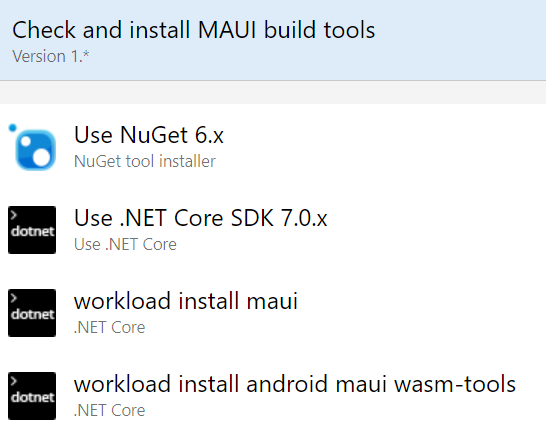
\includegraphics[width=\textwidth]{taskGroupMauiPrepare_light.png}}
        \caption{Zawartość grupy zadań inicjujących środowisko}
        \label{img:taskGroupMauiPrepare}
    \end{minipage}
\end{figure}

\newpage

O ile ten pipeline spełniał swoje zadanie na minimalnym poziomie, czyli przygotowywał potrzebne narzędzia 
oraz kompilował i podpisywał aplikację skierowaną na system Android, to jednak jego efektywność i prostota 
utrzymania pozostawiały wiele do życzenia.

Pierwszym z zarzutów jest zbędne wykonanie \verb|dotnet restore| - choć narzut pracy 
jest stosunkowo niewielki, wprowadza kolejny punkt zaczepienia do zadania pytania "czy mogę to zmienić?", 
które mogłaby zadać osoba bliżej niezaznajomiona z działaniem narzędzia.

Drugim problemem okazał się brak wykorzystania zmiennych, które wraz z parametryzacją procesu 
pozwoliłyby na uczynienie go bardziej elastycznym i uniwersalnym. 
Pomimo skorzystania z bezpiecznych zmiennych w procesie podpisywania pliku APK, 
byłem w stanie skorzystać wyłącznie z jednego, wcześniej przygotowanego zestawu danych, 
którego nie mogłem zmienić przed wywołaniem pipeline'a.

% \begin{figure}[hb]
%     \centering
%     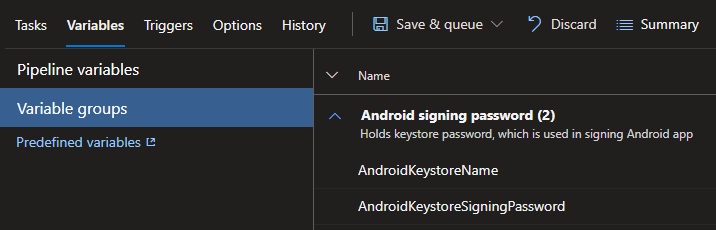
\includegraphics[width=0.75\textwidth]{variableGroups.png}
%     \caption{Predefiniowane zmienne przechowujące nazwę oraz hasło podpisujące certyfikat}
%     \label{img:variableGroups}
% \end{figure}


\subsubsection{Wersja YAML}
Finalną wersję pipeline'a umieściłem bezpośrednio w repozytorium jako pliki YAML w folderze \verb|CI|.
Korzystając z możliwości Azure podzieliłem duży plik zawierający wszystkie kroki 
na pomniejsze template'y (szablony), które mogę ponownie wykorzystać w dowolnie dużej 
ilości i kolejności.

Cała struktura zadań podzielona jest na kilka grup - tworząc je możemy zacząć od etapów (ang. stage), 
wewnątrz nich zawrzeć kilka jobów (prac, zadań), które składają się z kroków wykonania (ang. steps).


\begin{figure}[ht]
    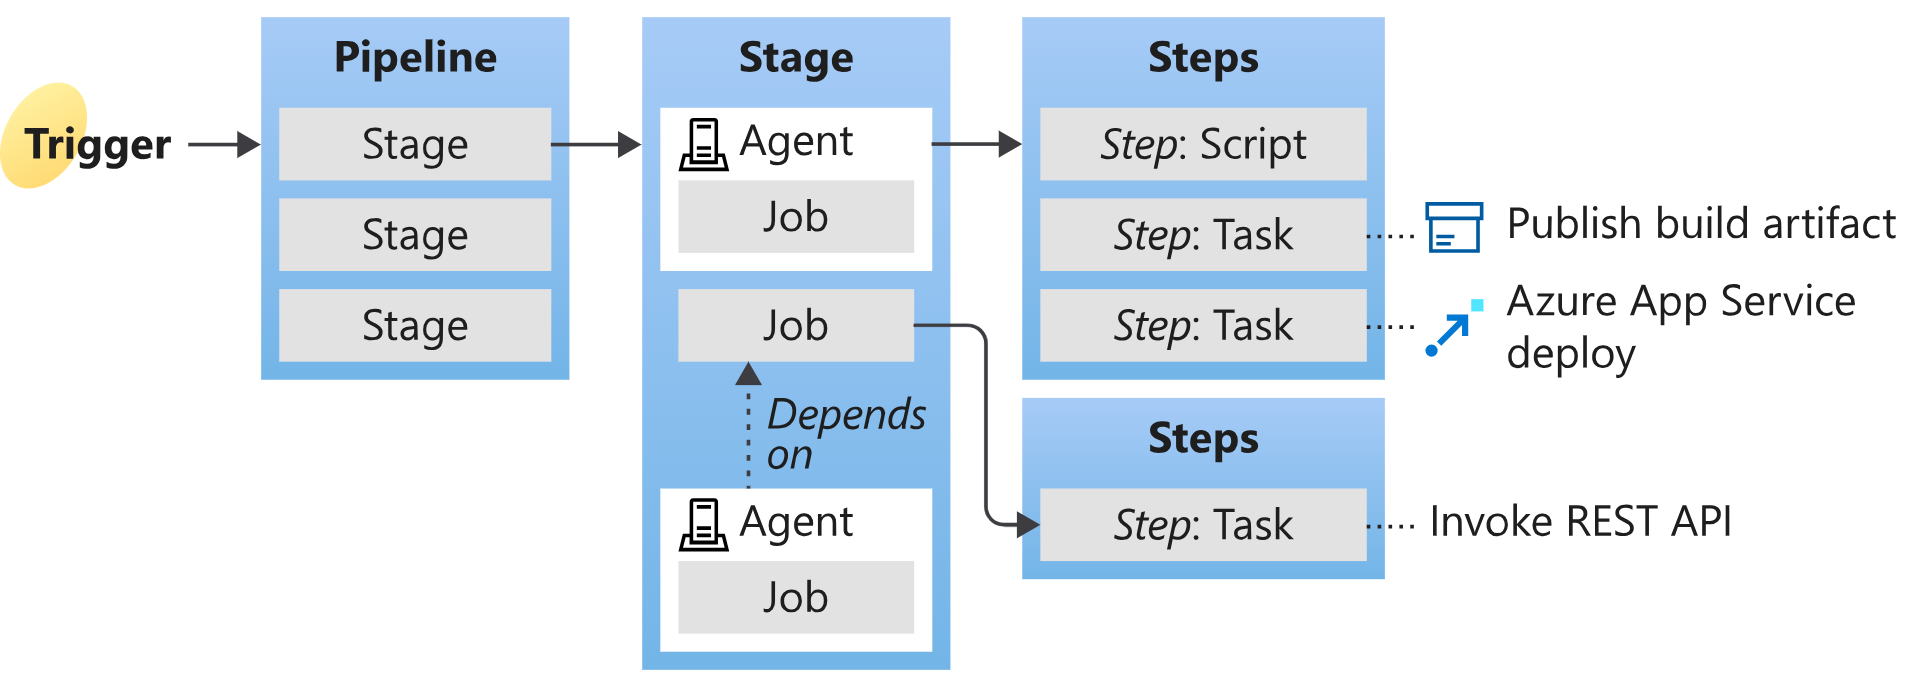
\includegraphics[width=\textwidth]{pipelineSchemaAzure.png}
    \caption{Hierarchia etapów i zadań w Azure~\cite{pipelineSchemaAzure_source}}
    \label{img:pipelineSchemaAzure}
    
\end{figure}


    \section{Podsumowanie i wnioski}
Nowoczesny rozwój oprogramowania jest bardzo dynamiczny, dociera już do nawet 
najmniejszych odbiorców prywatnych czy mikrofirm. W przypadku dużych organów 
skorzystanie z takich usług jest kluczowe.

Dla zapewnienia jak najwyższej jakości usług, wykorzystanie przedstawionych 
narzędzi CI/CD jest bardzo istotne. Problemy dystrybucji, środowisk oraz 
czuwania wprowadzeniem zmian zostają w prosty sposób zautomatyzowane, 
co obniża koszty obsługi i zwiększa dostępność takich serwisów.

Celem tej pracy było zaprezentowanie przygotowanego rozwiązania CI/CD, 
wyjaśnienie powodu jego zastosowania, sposobu działania i najistotniejszych 
elementów składowych pipeline'a. Aplikacja "Navigator" posłużyła jako 
przykład dzięki swoim wieloplatformowym możliwościom, ale również zwróciła 
uwagę na istotność dobrych praktyk programistycznych, takich jak zastosowanie 
wzorców projektowych lub odpowiedniego stworzenia architektury projektu.
W rezultacie cel pracy został osiągnięty.

Aplikacja "Navigator" może być w dalszym stopniu rozwijana, nie tylko pod 
względem naprawy błędów czy zmiany jej wyglądu, ale również dodawania 
nowych funkcjonalności. Skonfigurowany pipeline bez wątpienia ułatwi 
i przyspieszy wprowadzanie zmian, a uporządkowana architektura 
zmniejszy ilość trudności przy czytaniu kodu przez nowych programistów.
W celu zmniejszenia ilości wykonywanych operacji, dobrym pomysłem byłoby 
zaimplementowanie zapisywania wygenerowanych widoków HTML w pamięci 
oraz wprowadzenie systemu wersjonowania map.
W celu zmniejszenia ruchu sieciowego, istnieje również opcja 
dodania obsługi lokalnej kopii biblioteki Leaflet.

Modularna struktura plików \verb|.yaml| pozwala na bezproblemowe 
dodanie kolejnych etapów oraz kroków do procesu wydania, 
a ich czytelność ułatwi diagnozowanie ewentualnych błędów.


    \section{Dodatkowe źródła i przydatne materiały} \label{dodatkoweZrodla}
W tej sekcji umieszczam przydatne linki wraz z krótkimi opisami ich zawartości,
które przyczyniły się w istotny sposób do poprawy jakości pracy, ale nie wypisałem ich w cytowaniach,
ze względu na brak bezpośredniego cytowania.

\begin{itemize}
    \item YouTube - .NET MAUI for Beginners \\
        oficjalny poradnik, który wstępnie oprowadził mnie po zastosowaniach i ob\-słu\-dze frameworka. \\
        \href{https://youtube.com/playlist?list=PLdo4fOcmZ0oUBAdL2NwBpDs32zwGqb9DY}%
        {youtube.com/playlist?list=PLdo4fOcmZ0oUBAdL2NwBpDs32zwGqb9DY}\\
        (Dostęp: 29.12.2023)
    \item YouTube - Signing \& Versioning Android Apps\\
        Przydatny poradnik do podpisywania aplikacji wewnątrz pipeline'a.\\
        \href{https://youtube.com/watch?v=s1grtSSIRVA}{youtube.com/watch?v=s1grtSSIRVA}
        (Dostęp: 29.12.2023)
    \item ZipAlign - narzędzie Android SDK\\
        Opis i sposób użycia narzędzia \verb|zipalign| \\
        \href{https://developer.android.com/tools/zipalign}{developer.android.com/tools/zipalign}\\
        (Dostęp: 29.12.2023)
    \item Importowanie bibliotek za pomocą mechanizmu refleksji\\
        Krótka prezentacja sposobu importowania dynamicznych bibliotek wewnątrz uruchomionej aplikacji \\
        \href{https://learn.microsoft.com/en-us/dotnet/framework/reflection-and-codedom/how-to-load-assemblies-into-the-reflection-only-context}%
        {learn.microsoft.com/en-us/dotnet/framework/reflection-and-codedom/how-to-load-assemblies-into-the-reflection-only-context}\\
        (Dostęp: 29.12.2023)
    \item Material Symbols - biblioteka darmowych ikon od Google\\
        W mojej aplikacji skorzystałem z kilku ikon udostępnianych przez firmę posiadającą i stale 
        rozwijającą Androida, czyli właśnie Google. Mnogość możliwości ich personalizacji 
        oraz wygoda korzystania (możliwość pobrania całej paczki lub tylko jej części, 
        dostępność formatów wektorowych lub ich rastrowych odpowiedników) sprawiła, 
        że z przyjemnością użyję jej ponownie.
        \href{https://fonts.google.com/icons}{fonts.google.com/icons}
        (Dostęp: 29.12.2023)
\end{itemize}


    \listoffigures
    \newpage

    \newgeometry{top=3cm}
    \printbibliography[title={Bibliografia}]
    \restoregeometry
    \textbf{Oświadczenie autora pracy}

Ja, niżej podpisany, \\
Kacper Krzysztof Hałaczkiewicz, \\
autor pracy dyplomowej pt. "PRZYGOTOWANIE KOMPLETNEGO \\
ROZWIĄZANIA CI/CD NA PODSTAWIE APLIKACJI Z .NET MAUI", \\
numer albumu: 338889, \\
student Wydziału Nauk Ścisłych i Technicznych Uniwersytetu Śląskiego w Katowicach, \\
kierunku studiów Informatyka Stosowana, \\
oświadczam, że ww. praca dyplomowa: 
\begin{itemize}
    \item została przygotowana przeze mnie samodzielnie, 
    \item nie narusza praw autorskich w rozumieniu ustawy z dnia 4 lutego 1994 r. o prawie autorskim i prawach pokrewnych (tekst jednolity Dz. U. z 2006 r. Nr 90, poz. 631, z późn. zm.) oraz dóbr osobistych chronionych prawem cywilnym, 
    \item nie zawiera danych i informacji, które uzyskałem w sposób niedozwolony, nie była podstawą nadania stopnia doktora nauk, dyplomu wyższej uczelni lub tytułu zawodowego ani mnie, ani innej osobie. 
\end{itemize}

Oświadczam również, że treść pracy dyplomowej zamieszczonej przeze mnie w Archiwum Prac Dyplomowych 
jest identyczna z treścią zawartą w wydrukowanej wersji pracy. \\
\textbf{Jestem świadomy odpowiedzialności karnej za złożenie fałszywego oświadczenia.}



\end{document}